\section{R2U2 Hardware Implementation in VHDL}
The VHDL version of R2U2 has two modes of operation: an offline mode and an online mode. The offline mode reasons over a logged trace of sensor data, which can be used to validate an MLTL formula over a trace and for regression testing over a variety of benchmark formulas \& traces. Conversely, the online version reads streaming sensor data, which is read directly from a data bus or a custom preprocessing hardware block, and transmits its verdict via UART to a host PC.

\subsection{Getting Started}
Note that this version of R2U2 was designed in Xilinx's Vivado 2017.2. Additionally, the following are needed to compile this version of R2U2
\begin{itemize}
	\item \textbf{Python:} Version 2.6 (or greater) \textbf{and} Version 3.6 (or greater)
	\item \textbf{Packages:} pyserial, ply
\end{itemize}

\subparagraph{R2U2-VHDL Tool-chain Flow:} Figure \ref{fig:r2u2hwFlow} shows the tool-chain flow of the VHDL version of R2U2. To use this version of R2U2, the user needs to supply R2U2 with an MLTL formula and a custom VHDL file for interfacing with a data bus and/or a set of sensors. If the user wishes to use the offline mode, they must also supply a trace of sensor data. The user will start by compiling their MLTL formula into an Assembly File (\textit{.ftasm}). Within this step, the SCQ size (amount of memory required for R2U2's instruction sequence) is determined and stored in a \textit{.ftscq} file. The \textit{.ftasm} must then be compiled into a Binary Instruction (\textit{.ftm}) and a Binary Instruction Interval (\textit{.fti}) file. In parallel, the user must configure R2U2-VHDL's parameters to match those of the desired sensor values. This is done by modifying the \textit{config.py}, \textit{inputs.py}, and the \textit{.ast} file. Additionally, the user must incorporate their own custom hardware for interfacing their current system with R2U2 to run online. This version of R2U2 can also be run offline, i.e., fed a trace of sensor data via UART. 

\begin{figure}[H]
	\begin{center}
	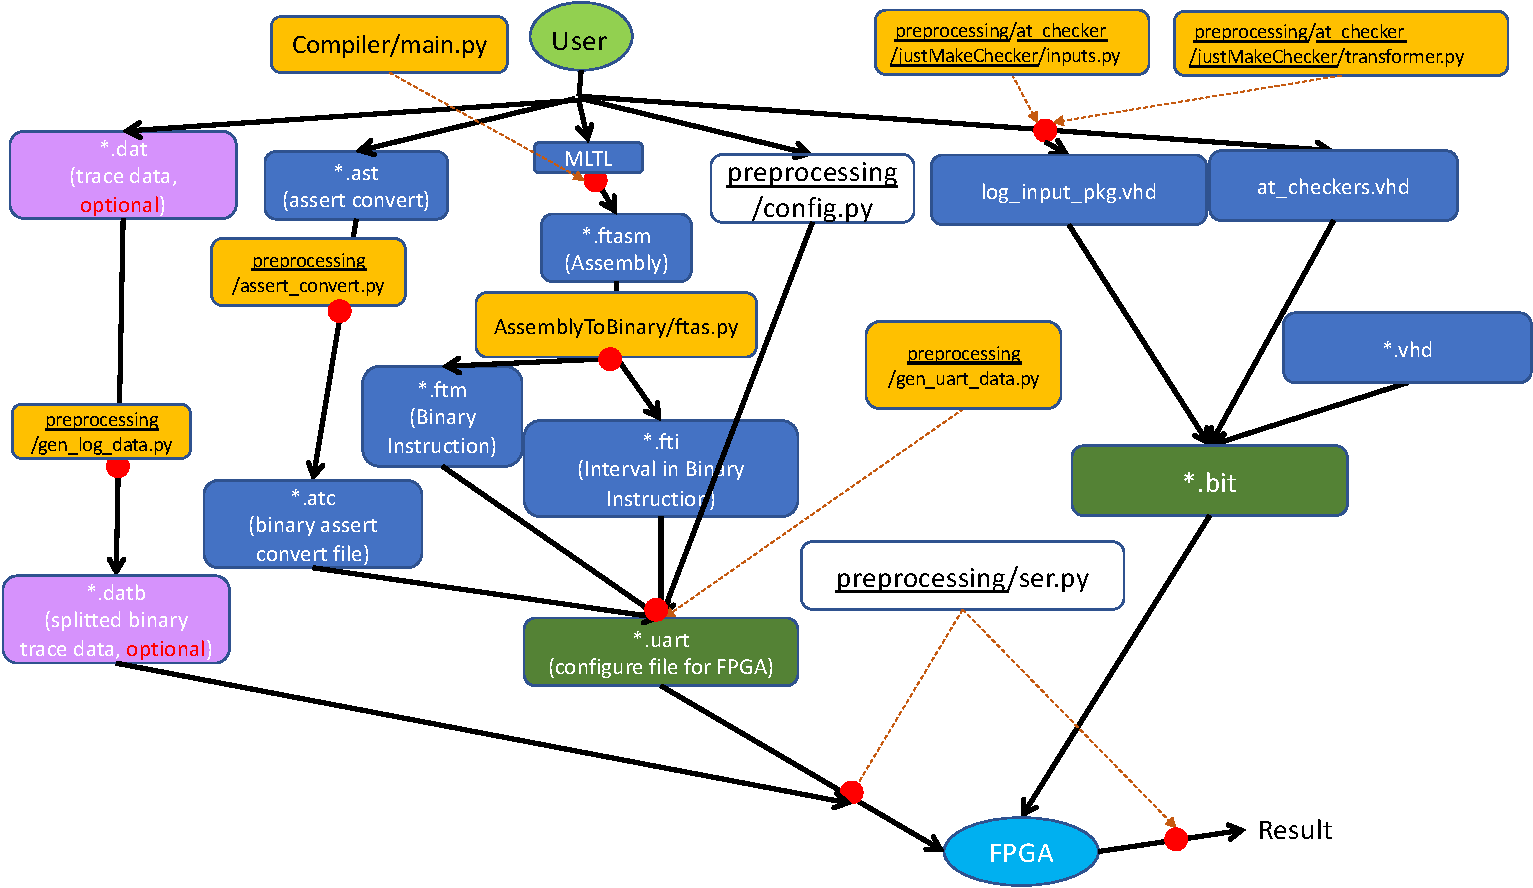
\includegraphics[scale=0.5]{fig/r2u2_fpga_flow.pdf}
	\caption{The flow of how the VHDL version of R2U2 is compiled and deployed. 
	\label{fig:r2u2hwFlow}} 
	\end{center}
\end{figure}

\subsection{User Specified Files}
This section describes the different files users need to provide or modify to launch the hardware version of R2U2. 
\subsubsection{Configuration File}
\label{config}
The first step is to tailor the \textit{config.py} file (located within the \textbf{../tools/preprocessing} directory) for the specific project. The following parameters can be modified within this file:
\begin{itemize}
	\item \textbf{SENSOR\_DATA\_WIDTH:} The maximum number of bits in the input to the atomic checkers. The upper-bound of this parameter is 32-bits.
	\item \textbf{NUM\_OF\_SENSOR:} The number of sensor inputs interfacing with R2U2.
	\item \textbf{SERIAL\_RUN\_MODE:} The mode in which R2U2 will execute.
	\begin{itemize}
		\item \textbf{self\_sensing:} R2U2 will execute based on the sensor input values streamed from external hardware.
		\item \textbf{read\_log:} R2U2 will execute based on the trace file given in \textbf{SENSOR\_DATA\_FILE}.
		\item \textbf{type\_input:} R2U2 will execute based on the binary values transmitted via the CLI.
	\end{itemize}
	\item \textbf{DATA\_SAMPLE\_NUMBER:} The number of time stamps R2U2 will execute across a \textbf{read\_log} trace.
\end{itemize}

\subsubsection{MLTL Formula}
\label{HWmltlFormula}
The MLTL formula that R2U2 will reason over must be implemented in one of two ways: either written and saved into the \textit{main.py} file (located within the \textbf{tools/Compiler} directory) or entered directly into the CLI when compiling the \textit{.ftasm} assembly file. In either case the syntax for the MLTL formula is identical and an example of an MLTL formula is shown in Table \ref{HWmltlFormulaTable}. Note that the only difference is how special characters are labeled in the CLI: they must be proceeded with a `` $\setminus$ ''. Additionally, the syntax for the MLTL formulas can be seen in Table \ref{HWsyntaxMLTL}.

\begin{table}[H]
	\caption{An example of an MLTL formula and the syntactical conversion into either the file type or the CLI.}
	\label{HWmltlFormulaTable}
	\begin{center}
	\begin{tabular}{l | l}
		\hline
		\hline
		\textbf{Type} & \textbf{Formula Format}\\
		\hline
		Expression & $G_{0,3}((a_0\bigwedge a_1)\bigwedge (a_2 \bigwedge s_3))$\\
		\textit{main.py} & MLTL = ``G[0,3]((a0 \& a1) \& (a2 \& a3))''\\
		CLI & G[0,3]((a0$\setminus$\&a1) $\setminus$\&(a2$\setminus$\&a3))\\
		\hline
		\hline
	\end{tabular}
	\end{center}
\end{table}

\begin{table}[H]
	\caption{The format for the MLTL operators, which are used to create a single MLTL formula which can either be saved to the \textit{main.py} file or incorporated into the CLI. Note that $E$1 and $E$2 denote that that parameter can be either a single atomic or an expression, to allow for more complex formulas.}
	\label{HWsyntaxMLTL}

	\begin{center}
	\begin{tabular}{l | c | c | c | c | c | c}
		\hline
		\hline
		\textbf{Expression} & \textit{NOT} & \textit{Next} & \textit{Until} & \textit{Global} & \textit{AND} & \textit{OR}\\
		\hline
		\textbf{Syntax} & !$E$1 & $XE$1 & $E$1 $U$[$t_i$,$t_f$] $E$2 & $G$[$t_i$,$t_f$] $E$1 & $E$1 \& $E$2& $E$1 $|$ $E$2\\
		\hline
		\textbf{Precedence} & 1 & 1 & 2 & 2 & 3 & 3\\
		\hline
		\hline
	\end{tabular}
	\end{center}
\end{table}

\subsubsection{Configuring Atomic Checkers}
\label{ConfigAC}

\subparagraph{Atomic Checker File:}
Since R2U2 reasons over Boolean values, sensor values must be pre-processed into Boolean atomics. This is done by R2U2's Atomic Checkers, which can perform fixed-point addition, subtraction, and a power-of-two multiplication/division on no more than two sensor values. Then it performs a comparison operation against a predefined value, to determine its Boolean output.

Each atomic in R2U2's MLTL formula will have its own Atomic Checker Block in hardware. The \textit{inputs.py} script in the \textbf{tools/preprocessing} directory allows users to specify the bit-length, name, and units of their sensor signals. From there, the \textit{transformer.py} script can be executed to automatically generate the VHDL file for R2U2 with the specified number of atomic checker blocks.

\subparagraph{Atomic Checker Block:}
The hardware for an atomic checker block must be customized for each instantiation. within the design. A diagram for this hardware block can be seen in Fig. \ref{fig:ACB}.

\begin{figure}[H]
	\begin{center}
	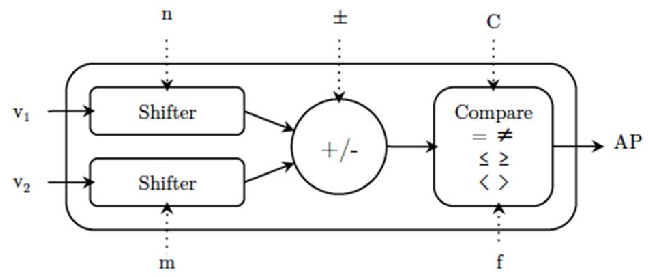
\includegraphics[scale=0.5]{fig/AtomicCheckerBlock.pdf}
	\caption{A high-level schematic of the configurable Atomic Checker block.
	\label{fig:ACB}} 
	\end{center}
\end{figure}

To configure each checker within the design, the user must modify the \textit{input.ast} file within the \textbf{tools/preprocessing} directory. In this file, each line indicates the configuration for each atomic checker. The syntax for this file reads as follows:

\begin{equation}
	C;n;m;Op;F
\end{equation} 
where $C$ is the integer value used in the comparison, $n$ \& $m$ are the number of arithmetic shifts performed on $v_1$ \& $v_2$, respectively, $Op$ is the mathematical operation performed on the post-shifted input values, and $F$ is the selected comparison function for the block. The syntax for the comparison \& arithmetic operations can be seen in Table \ref{syntaxACB}. Note that the shift operations can be used to perform fixed-point multiplication or division by powers of 2. 

\begin{table}[H]
	\caption{The valid comparison \& arithmetic operations the Atomic Checker block can perform as well as their respective syntax for the \textit{input.ast} file.
	\label{syntaxACB}}
	\begin{center}
	\begin{tabular}{l | c | c | c | c | c | c}
		\hline
		\hline
		&\multicolumn{6}{c}{\textbf{Comparison Operations}}\\
		\hline
		\textbf{Operation} & $=$ & $\neq$ & $\geq$ & $>$ & $\leq$ & $<$ \\
		\hline
		\textbf{Syntax} & \textit{EQU} & \textit{NEQ} & \textit{GEQ} & \textit{GRE} & \textit{LEQ} & \textit{LES}\\
		\hline
		\hline
		&\multicolumn{6}{c}{\textbf{Arithmetic Operations}}\\
		\hline
		\textbf{Operation} & \multicolumn{2}{c}{$v_1+v_2$} & \multicolumn{2}{c}{$v_1-v_2$} &\multicolumn{2}{c}{$|v_1-v_2|$} \\
		\hline
		\textbf{Syntax} & \multicolumn{2}{c}{\textit{ADD}} & \multicolumn{2}{c}{\textit{SUB}} & \multicolumn{2}{c}{\textit{DIF}}\\
		\hline
		\hline
	\end{tabular}
	\end{center}
\end{table}

After configuring the \textit{input.ast} file for the given project, execute the script \textit{assert\_convert.py} script to automatically convert the configurations within the \textit{input.ast} file into a binary format suitable for the hardware.


\subsubsection{Modifying the VHDL Files}
\label{ModVHDL}
This section describes R2U2's VHDL files that a user would need to modify for their own sensors to be integrated with the hardware version of R2U2. The atomic checker blocks of R2U2 are configurable for up to a 32-bit fixed-point value. Thus, the sensor data must be passed to R2U2 as a fixed-point value. This can be done by connecting R2U2 directly to a software configurable register or a custom hardware preprocessing component. Note that a basic outline for interfacing R2U2 with a custom hardware component is given, but there may be additional modifications necessary for interfacing software registers to R2U2, i.e., additional files for interfacing with the CPU via AXI to allow for software configurable registers to hold sensor values.

\subparagraph{sensor\_log.vhd:} The \textit{sensor\_log.vhd} file (in the \textbf{R2U2\_HW/customize} directory) must be customized for the desired project. Note that this is where R2U2 registers the incoming sensor data and stores it into a singular register \textit{\textbf{log\_data}} of \textbf{LOG\_DATA\_WIDTH}, which is a concatenation of the one or more sensor's fixed-point data. Currently, R2U2's \textit{\textbf{log\_data}} register stores the sensors in descending order, with the order specified in the \textit{inputs.py} file (in the \textbf{tools/preprocessing} directory). 

\begin{figure}[H]
	\begin{center}
	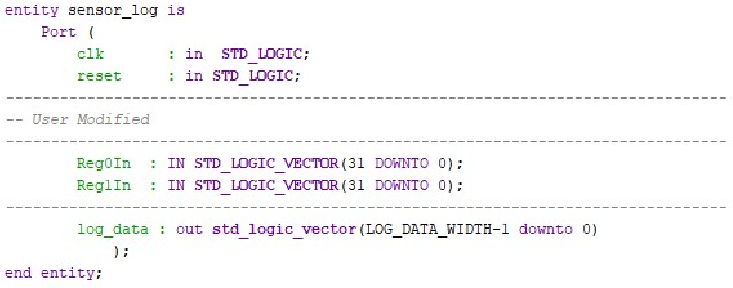
\includegraphics[scale=0.5]{fig/r2u2_hw_sensorLog_entity.pdf}
	\caption{A screenshot of \textit{sensor\_log.vhd}'s entity block, showing where the user will configure the file's input parameters. 
	\label{fig:r2u2hwSLentity}} 
	\end{center}
\end{figure}

\begin{figure}[H]
	\begin{center}
	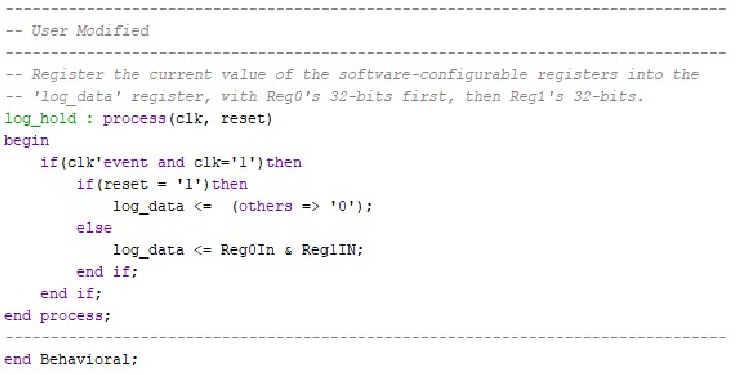
\includegraphics[scale=0.5]{fig/r2u2_hw_sensorLog_arch.pdf}
	\caption{A screenshot of \textit{sensor\_log.vhd}'s architecture block, showing where the user will configure the file's process block so that the \textit{\textbf{log\_data}} register is the concatenation of all the sensor values. 
	\label{fig:r2u2hwSLarch}} 
	\end{center}
\end{figure}

\subparagraph{echo.vhd:} The file \textit{echo.vhd} (located in the \textbf{R2U2\_HW/uart} directory) instantiates the file \textit{sensor\_log.vhd}. Thus, we must modify this file, specifically its entity block, the component declaration, and the component instantiation, as seen in Fig. \ref{fig:r2u2hwEchoEnt}, \ref{fig:r2u2hwEchoCom}, and \ref{fig:r2u2hwEchoInst}.

\begin{figure}[H]
	\begin{center}
	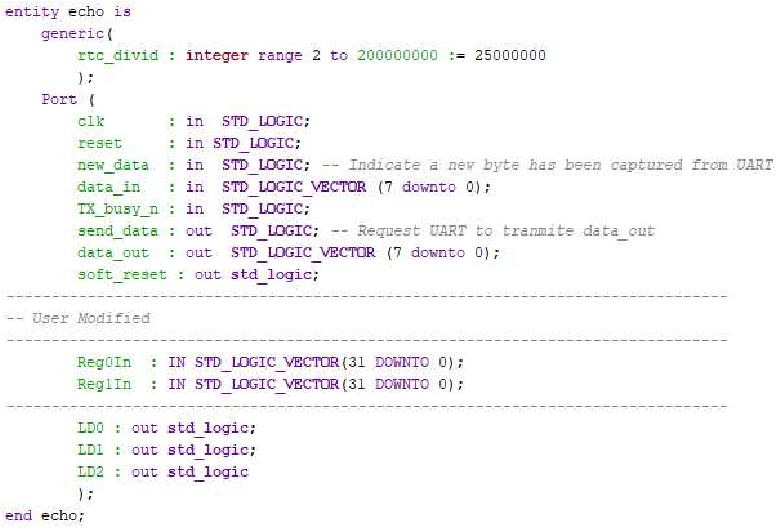
\includegraphics[scale=0.5]{fig/r2u2_hw_echo_entity.pdf}
	\caption{A screenshot of \textit{echo.vhd}'s entity block, showing where the user will configure the file's inputs to match those of \textit{sensor\_log.vhd}
	\label{fig:r2u2hwEchoEnt}} 
	\end{center}
\end{figure}

\begin{figure}[H]
	\begin{center}
	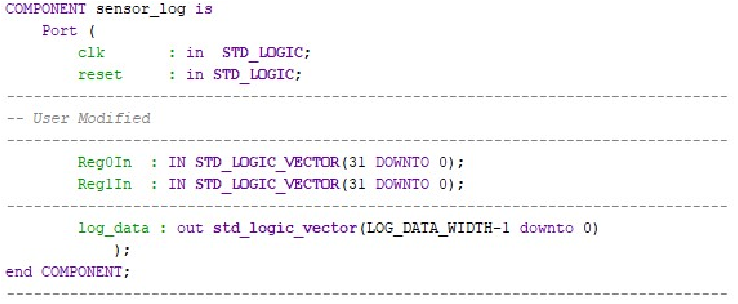
\includegraphics[scale=0.5]{fig/r2u2_hw_echo_component.pdf}
	\caption{A screenshot of \textit{echo.vhd}'s component declaration, showing where the user will configure the \textbf{sensor\_log} component's input signals to match those of the \textit{sensor\_log.vhd}'s entity block.
	\label{fig:r2u2hwEchoCom}} 
	\end{center}
\end{figure}

\begin{figure}[H]
	\begin{center}
	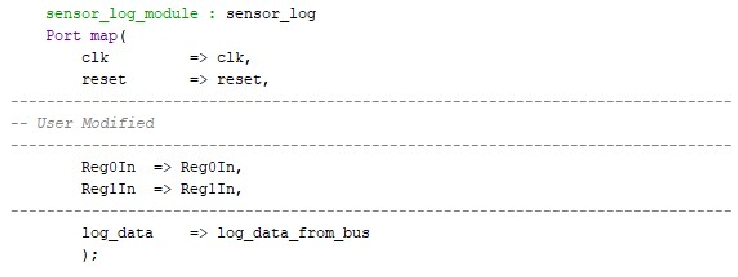
\includegraphics[scale=0.5]{fig/r2u2_hw_echo_inst.pdf}
	\caption{A screenshot of \textit{echo.vhd}'s instantiation of the \textbf{sensor\_log}, showing where the user will configure the signals to match those within their current design.
	\label{fig:r2u2hwEchoInst}} 
	\end{center}
\end{figure}

\subparagraph{process\_data.vhd:} The file \textit{process\_data.vhd} (located in the \textbf{R2U2\_HW/uart} directory) instantiates the file \textit{echo.vhd}. Thus, we must modify this file, specifically its entity block, the component declaration, and the component instatiation, as seen in Fig. \ref{fig:r2u2hwProEnt}, \ref{fig:r2u2hwProCom}, and \ref{fig:r2u2hwProInst}.

\begin{figure}[H]
	\begin{center}
	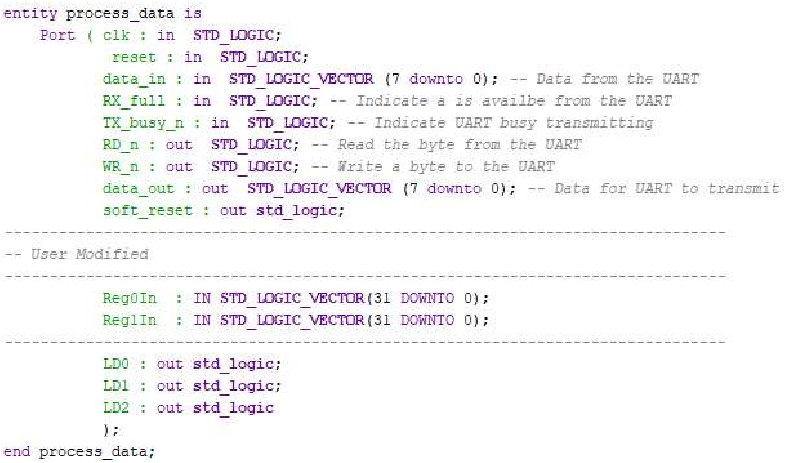
\includegraphics[scale=0.5]{fig/r2u2_hw_process_entity.pdf}
	\caption{A screenshot of \textit{process\_data.vhd}'s entity block, showing where the user will configure the file's inputs to match those of \textit{echo.vhd}
	\label{fig:r2u2hwProEnt}} 
	\end{center}
\end{figure}

\begin{figure}[H]
	\begin{center}
	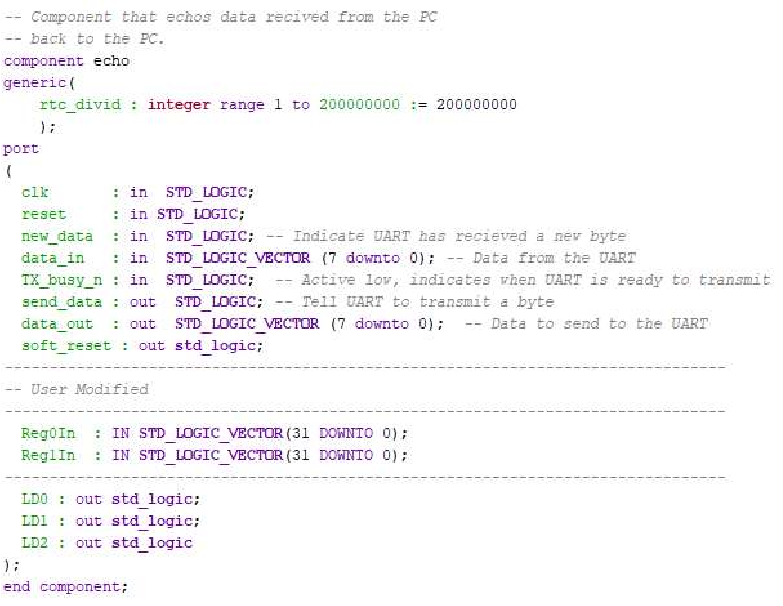
\includegraphics[scale=0.5]{fig/r2u2_hw_process_component.pdf}
	\caption{A screenshot of \textit{process\_data.vhd}'s component declaration, showing where the user will configure the \textbf{echo} component's input signals to match those of the \textit{echo.vhd}'s entity block.
	\label{fig:r2u2hwProCom}} 
	\end{center}
\end{figure}

\begin{figure}[H]
	\begin{center}
	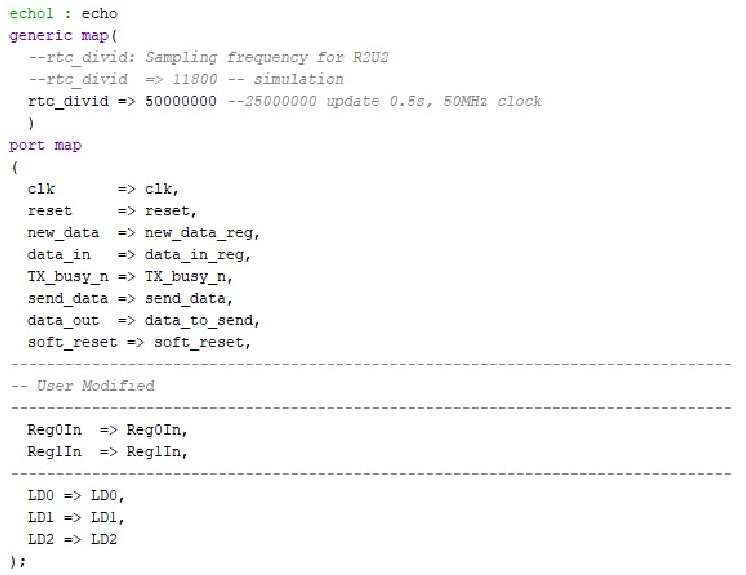
\includegraphics[scale=0.5]{fig/r2u2_hw_process_inst.pdf}
	\caption{A screenshot of \textit{process\_data.vhd}'s instantiation of the \textbf{echo}, showing where the user will configure the signals to match those within their current design.
	\label{fig:r2u2hwProInst}} 
	\end{center}
\end{figure}

\subparagraph{MP1.vhd:} The file \textit{MP1.vhd} (located in the \textbf{R2U2\_HW/uart} directory) is the top-level file for the design, i.e., this file connects all the other relevant files for the hardware version of R2U2. Thus, this file instantiates both the \textit{process\_data.vhd} file and the user's custom hardware file. Thus, we must modifty its entity block, the component declarations, the signal declarations, and the component instantiations, as seen in Fig. \ref{fig:r2u2hwMP1Ent}, \ref{fig:r2u2hwMP1Comp}, \ref{fig:r2u2hwMP1customComp}, \ref{fig:r2u2hwMP1customSig}, \ref{fig:r2u2hwMP1Inst}, and \ref{fig:r2u2hwMP1customInst}. 

\begin{figure}[H]
	\begin{center}
	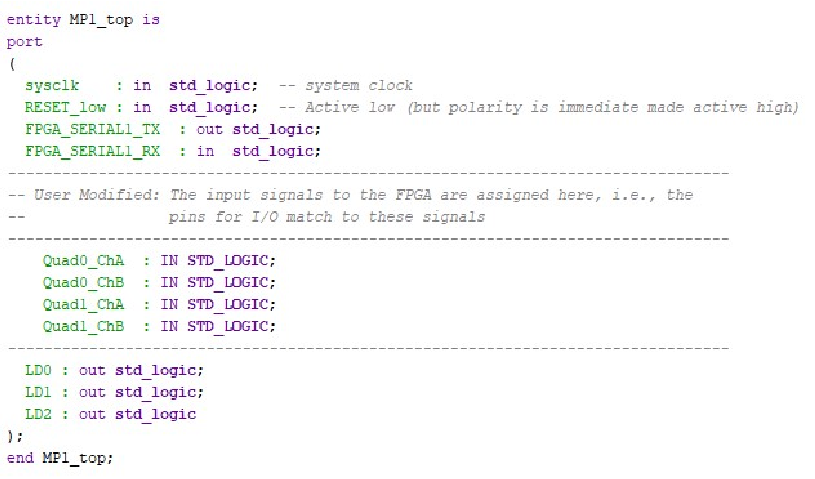
\includegraphics[scale=0.5]{fig/r2u2_hw_mp1_entity.pdf}
	\caption{A screenshot of \textit{MP1.vhd}'s entity block, showing where the user will configure the file's inputs from the FPGA's pins.
	\label{fig:r2u2hwMP1Ent}} 
	\end{center}
\end{figure}

\begin{figure}[H]
	\begin{center}
	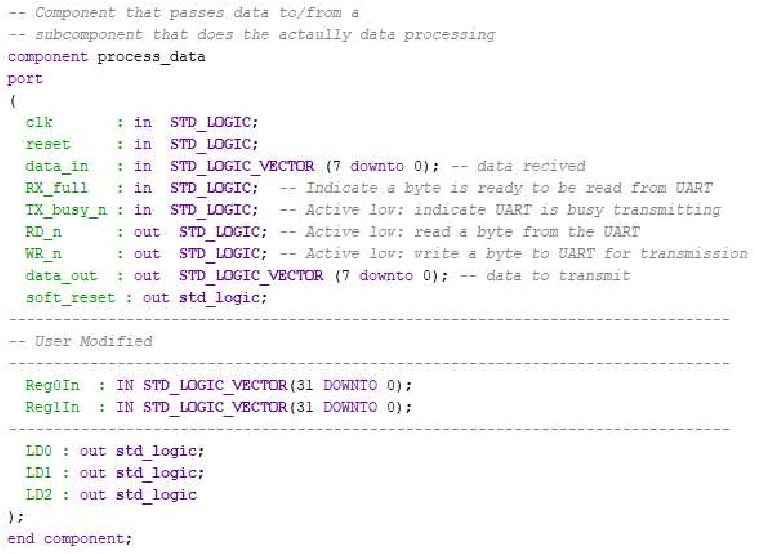
\includegraphics[scale=0.5]{fig/r2u2_hw_mp1_component.pdf}
	\caption{A screenshot of \textit{process\_data.vhd}'s component declaration, showing where the user will configure the \textbf{process\_data} component's input signals to match those of the \textit{process\_data.vhd}'s entity block.
	\label{fig:r2u2hwMP1Comp}} 
	\end{center}
\end{figure}

\begin{figure}[H]
	\begin{center}
	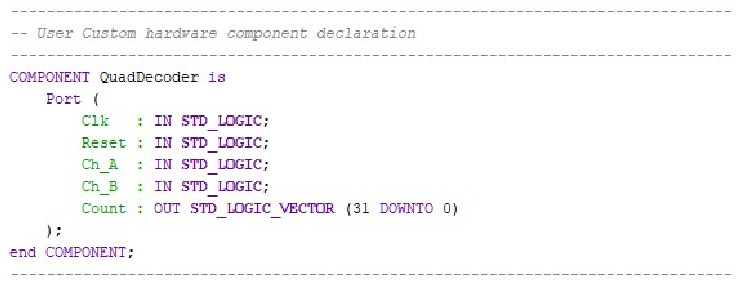
\includegraphics[scale=0.5]{fig/r2u2_hw_mp1_custom_comp.pdf}
	\caption{A screenshot of a custom hardware's component declaration.
	\label{fig:r2u2hwMP1customComp}} 
	\end{center}
\end{figure}

\begin{figure}[H]
	\begin{center}
	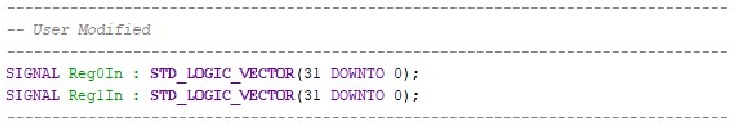
\includegraphics[scale=0.5]{fig/r2u2_hw_mp1_custom_signals.pdf}
	\caption{A screenshot of the custom signals \textbf{Reg0In} and \textbf{Reg1In}, which must be declared inside \textbf{MP1}'s architecture block to connect the instantiations of the custom hardware to the \textbf{process\_data} instantiation.
	\label{fig:r2u2hwMP1customSig}} 
	\end{center}
\end{figure}

\begin{figure}[H]
	\begin{center}
	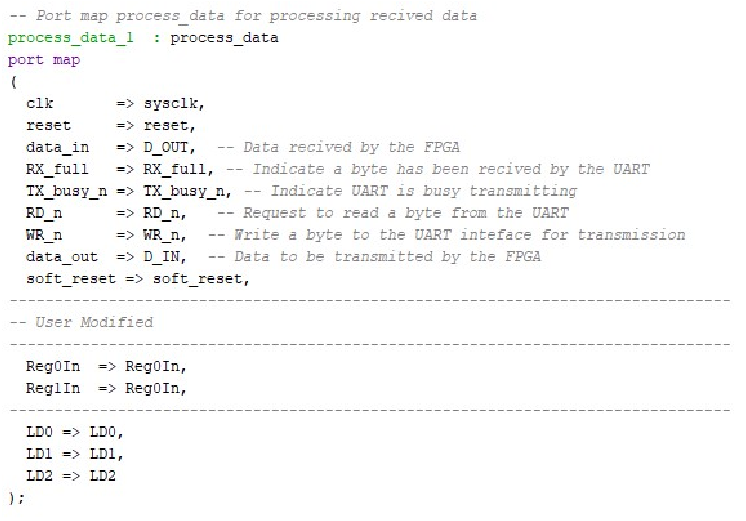
\includegraphics[scale=0.5]{fig/r2u2_hw_mp1_inst.pdf}
	\caption{A screenshot of \textit{MP1.vhd}'s instantiation of the \textbf{process\_data}, showing where the user will configure the signals to match those within their current design.
	\label{fig:r2u2hwMP1Inst}} 
	\end{center}
\end{figure}

\begin{figure}[H]
	\begin{center}
	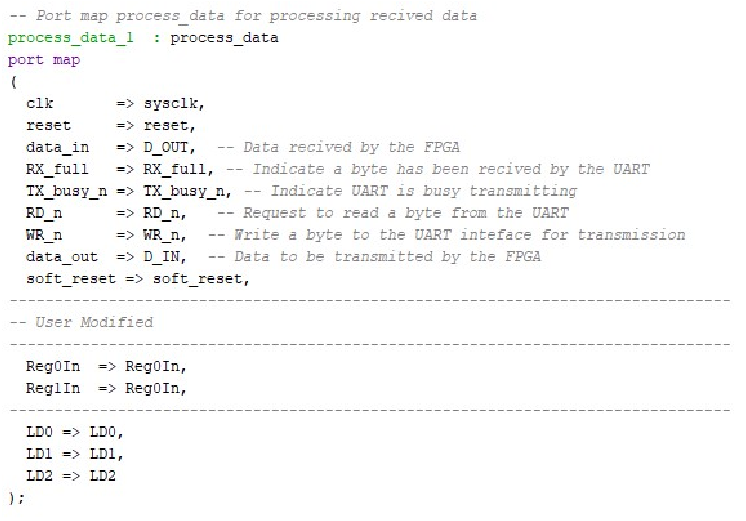
\includegraphics[scale=0.5]{fig/r2u2_hw_mp1_custom_inst.pdf}
	\caption{A screenshot of \textit{MP1.vhd}'s instantiation of the custom hardware, showing where the user will configure the signals to match those within their current design.
	\label{fig:r2u2hwMP1customInst}} 
	\end{center}
\end{figure}

\subsection{Running R2U2-VHDL}
\label{runR2U2}
\begin{enumerate}
% ***** Step #1 ***** 
	\item Navigate to the \textbf{tools/preprocessing} directory via
	\begin{lstlisting}[language=C]
	cd tools/preprocessing/
	\end{lstlisting}
	
% ***** Step #2 *****
	\item Modify \textit{config.py} file (refer to Section \ref{config}). Once modified to the desired settings, execute \textit{config.py} via:
	\begin{lstlisting}[language=C]
	python config.py
	\end{lstlisting}
	
% ***** Step #3 *****
	\item Navigate to the \textbf{tools} directory via:
	\begin{lstlisting}[language=C]
	cd ../
	\end{lstlisting}
	
% ***** Step #4 *****
	\item Modify \textit{main.py} in the \textbf{/tools/Compiler} directory with the desired MLTL formula. Note that the syntax for the MLTL formula must match that in Section \ref{HWmltlFormula}.
	
% ***** Step #5 *****
	\item Once the desired MLTL formula is in the \textit{main.py} file, convert the formula into the \textit{.ftasm} \& \textit{.ftscq} file structure via:
	\begin{lstlisting}[language=C]
	python Complier/main.py
	\end{lstlisting}
	
% ***** Step #6 *****
	\item Convert the \textit{.ftasm} assembly MLTL formula into the binary assembly \textit{.ftm} and binary assembly interval \textit{.fti} file structures via: 
	\begin{lstlisting}[language=C]
	cat tmp.ftasm | AssemblyToBinary/ftas.py tmp
	\end{lstlisting}
	
% ***** Step #7 *****
	\item Naviagate to the \textbf{preprocessing/at\_checker} directory via: 
	\begin{lstlisting}[language=C]
	cd preprocessing/at_checker
	\end{lstlisting}
	
% ***** Step #8 *****
	\item Modify the \textit{inputs.py} script to  the correct number \& bit-length of sensor inputs and create the correct number of atomic checker blocks. Run the \textit{transformer.py} script via: 
	\begin{lstlisting}[language=C]
	python transformer.py
	\end{lstlisting}
	
% ***** Step #9 *****
	\item Navigate back to the \textbf{tools/preprocessing} directory via: 
	\begin{lstlisting}[language=C]
	cd ../
	\end{lstlisting}
	
% ***** Step #10 *****
	\item Copy the \textit{at\_checkers.vhd} and \textit{log\_input\_pkg.vhd} files into the \textbf{R2U2\_HW/customize} directory via:
	\begin{lstlisting}[language=C]
	cp at_checkers.vhd log_input_pkg.vhd ../../../R2U2_HW/customize
	\end{lstlisting}
% ***** Step #11 *****
	\item Within the \textbf{tools/preprocessing} directory, modify the \textit{input.ast} file with the correct configurations for each atomic checker block. 

% ***** Step #12 *****
	\item Convert the \textit{input.ast} file into the \textit{res.atc} file via: 
	\begin{lstlisting}[language=C]
	python assert_convert.py
	\end{lstlisting}
	
% ***** Step #13 *****
	\item Within the \textbf{/R2U2\_HW/customize} directory, modify the \textit{sensor\_log.vhd} file to store the sensor values within the its \textit{log\_data} output register (as seen in Section \ref{ModVHDL}).
	
% ***** Step #14 *****
	\item Launch Vivado and create a new project. Import the \textbf{R2U2\_HW} directory  as the source file, create a constraint file for the user's board (example one - \textit{zybo.xdc} - is shown in the \textbf{R2U2\_HW/customize} directory), and choose the correct development board or FPGA (example one is the Zybo with the xc7z010 FPGA). In the \textbf{Sources} tab, set \textit{UART\_HW:MP1\_top} as the top-level file. Then synthesize \& generate the project's bitstream. Program R2U2 onto the FPGA.
	
% ***** Step #15 *****
	\item If using the \textbf{online mode} (\textbf{SERIAL\_RUN\_MODE:} self\_sensing), skip to next step. Else, if using \textbf{offline mode} (\textbf{SERIAL\_RUN\_MODE:} read\_log):
	\begin{enumerate}
		\item Modify \textit{sensor\_data.dat} with the sensor trace
		\item Convert the \textit{sensor\_data.dat} to a binary version the UART can transmit via:
	\begin{lstlisting}[language=C]
	python gen_log_data
	\end{lstlisting}
	\end{enumerate}


% ***** Step #16 *****
	\item Merge the \textit{.atc}, \textit{.ftm}, and \textit{.fti} files together into the \textit{.uart} file structure via: 
	\begin{lstlisting}[language=C]
	python gen_uart_data
	\end{lstlisting}

% ***** Step #16 *****
	\item From the \textbf{/tools/preprocessing} directory, launch a serial connection to the external serial-to-UART connection via: 
	\begin{lstlisting}[language=C]
	python ser.py
	\end{lstlisting}
	Note that this command must be launched using Version 2 of Python. It will not execute in Python 3.
	
\end{enumerate}

\clearpage
